
\documentclass[oneside,a4paper,titlepage]{article}
\usepackage{blindtext}
\usepackage[utf8]{inputenc}
\usepackage{verbatim} 
\usepackage{graphicx}
\usepackage{color}
\usepackage{float}
% hidelinks fjerner farvede kanter omkring links og refferencer
\usepackage[hidelinks]{hyperref}
\usepackage{lipsum}
\usepackage{pdfpages}

% Mappe hvori billeder ligger
\graphicspath{ {graphics/} }

% Tekst som står først i figur captions "{Figure/Figur} 3: Pixelering der fremkommer..."
\renewcommand{\figurename}{Figur}


% supresses errors during compilation
% \batchmode

\title{Ray Tracing}
\author{P1 B2-28}
\date{\today}

\begin{document}
\maketitle

\renewcommand{\abstractname}{Abstrakt}
\begin{abstract}
Abstract text placeholder, lorem ipsum dolor sit amet...
\end{abstract}

\tableofcontents
\clearpage

% sections
Selvom vi ikke tænker på det så ofte, så er lamper en stor del af vores hverdag. De står i vores hjem, på vores gader, på vores arbejdsplads - ja de er stort set overalt. Men hvorfor er lamper egentlig så udbredte? Det er de, fordi lamper bliver brugt til at skabe lys. Belysning kan bidrage til mange ting som at læse, arbejde mere koncentret eller til at skabe hygge og stemning i et rum, der ellers ville have været koldt og kedeligt. 
\newline Lamper findes i mange forskellige typer og mange forskellige steder. Der er læselamper, arbejdslamper, loftlamper, udendørslamper osv. og de tjener allesammen forskellige formål, men fælles for dem er, at de skaber lys steder hvor der ellers ikke ville have været lys. 
I dag findes der utroligt mange forskellige lampedesigns, og de er ikke allesammen lige gode. Dette vil sige at nogle lamper har meget dårlig belysning. Dette er et problem, da undersøgelser har vist at dårlig belysning kan føre til blandt andet øjenskader, hovedpine samt ondt i nakke og hals \cite{lys_konsekvenser}. Andre problemer kan også opstå, hvis en lampe har en for kraftig belysning, og derfor er blændende eller hvis f.eks en udendørs lampe ikke lyser tilstrækkeligt, og man derfor vælter, fordi man ikke kan se noget. 
Så selvom lamper spiller en stor rolle i vores hverdag, så er det vigtigt at kunne visualisere hvordan lys udbreder sig fra en lampe, så man kan undgå dårlig belysning. 
\newline Man kan derfor argumentere for at det essentielle ved en lampe ikke er dens design, men er det lys som den udsender, herunder mønster og farve, samt lysets indflydelse på indretning og belysning. Med afsæt i denne argumentation har vi derfor valgt at arbejde med visualisering af lyset fra lamper.

\subsection{Motivation}

Som studerende på software synes vi, at det kunne være interresant at arbejde med et håndterbart problem som der ville kunne findes en teknologisk løsning på. 
\newline Gruppens mål er derfor at finde et relevant problem indenfor visualisering af lyset fra lamper, og derudfra lave en teknologisk løsning på problemet. Som gruppe er vi motiveret af, at vi kan designe og implementere software med henblik på at finde en god løsning på et relevant problem. 

\subsection{Initierende problem}

I indledningen slog vi som gruppe fast, at vi gerne ville arbejde med visualisering af lyset fra lamper. På baggrund af vores viden om lys fra lamper, samt de erfaringer og diskussioner vi har foretaget os som gruppe, har vi valgt at opstille følgende initierende problem:

Forbrugeren kan ikke visualisere, hvordan lyset udbreder sig fra en lampe uden at købe og installere lampen.

\section{Problemanalyse}
\subsection{Begrebsligørelse}
Der er indtil videre blevet  argumenteret for relevansen af det initierende problem, og det er i den sammenhæng derfor nødvendigt at redegøre for nogle vigtige emner og ord indenfor problemfeltet. 

Formålet med dette afsnit er at beskrive vigtige begreber samt kort at give en beskrivelse af, hvordan de forskellige ord og begreber skal forstås i den videre rapport. Begreberne som fremgår i følgende afsnit danner grundlag for forståelsen af det initierende problem. Disse begreber er følgende: Forbruger, visualisering, lys og lamper.

% \subsubsection{Køber}
% En køber er en person, der køber et produkt eller tjenesteydelser \cite{ddo_forbruger}.  Køberen står altså i denne sammenhæng i modsætning til producenterne.
% I denne rapport opfattes køberen som den person der køber lampen. Det vil altså sige, at der i dette tilfælde ikke nødvendigvis er tale om personer der til dagligt bruger eller bliver påvirket af lampen.

\subsubsection{Forbruger}
En forbruger er en privatperson som køber et produkt eller tjenesteydelser. “Forbruge” betyder at “bruge noget”, og en forbruger køber derfor produkter med henblik på at tilfredsstille nogle behov \cite{forbrugerportalen}. En bevidst forbruger, vil derfor ofte lede efter produkter der opfylder deres behov. Man antages også for at være forbruger af en varer hvis man til daglig benytter sig af eller bliver påvirket af en given lampe. 

I vores rapport udvider vi definitionen af forbruger til, at en forbruger også kan være en erhvervsperson der køber en lampe til brug i virksomheden. Derudover hører en kunde også til under begrebet forbruger, da det er kunderne som køber lamperne. 

%\subsubsection{Sælger}
%En sælger er den person eller virksomhed der sælger et produkt eller %tjenesteydelser. I rapporten opfattes sælgeren som værende en person %eller virksomhed, der sælger lamper til forbrugeren. 

\subsubsection{Visualisering}
At visualisere, betyder at skabe et billede på baggrund af noget \cite{ddo_visualisering}. Dette kan til dels være tanker, som omsættes til billeder for det indre øje. Det kan også være en række data, som omsættes til billeder, så de er nemmere at forstå.
Visualisering kan være et redskab til at skabe en forståelse for det der visualiseres. Dette kan f.eks være prototyper af lamper, der kan give en forståelse for hvordan lyset udbreder sig fra en lampe. Derudover er der inden for computergrafik metoder til at skabe billeder på baggrund af 3D-modeller, så man f.eks. kan lave et delvist realistisk billede af en lampe, og på den måde få en forståelse for hvordan lampen ser ud i virkeligheden og hvordan dens lys udbredes. Forskellige teknologier til visualisering er uddybet senere i rapporten under afsnit \ref{sec:teknologianalyse}. 

\subsubsection{Lys}
Der er forskellige opfattelser af hvad lys det indebærer. Hvis vi tager udgangspunkt i Karsten Rottwitt, som er professor ved DTU fotonik, så påstår han at lys er:

“Lys er andet end synligt lys. For mig er lys et elektromagnetisk felt, som har en høj frekvens”
- Karsten Rottwitt\cite{def_lys}.

Han mener også, at der er en hårdfin grænse for hvornår lys kan betegnes som lys, denne grænse er dog først i spil når vi snakker om UV-lys og infrarødt lys \cite{def_lys}. 
Andre er ikke enige med Karsten Rottwitt om hvordan definitionen af lys er. Tager vi nu udgangspunkt i Britannica \cite{britannica_lys}, så betegnes lys, som magnetiske stråler, som det menneskelige øje kan opfange - Hvilket vil sige, lys med en bølgelængde mellem 380 og 750 nanometer, også kaldet synligt lys. 

Det er denne definition, som rapporten vil tage udgangspunkt i. Dette er valgt, da det er oplagt at kombinere synligt lys og lamper \cite{def_lys}.

Det lys som kommer fra en lampe, er selvfølgelig af forskellig kvalitet. Kvalitet kan ligesom lys, betegnes på mange måder, herunder kan vi snakke om hvorvidt en lyskilde er af god kvalitet, hvis den er energivenlig eller om det kun kommer an på hvor gode de er til at eftergive farvet lys. 
Afhængigt af hvor man skal bruge lyset, kan nogle former for lys være bedre egnet end andre. Her menes der om hvorvidt lyset skal være varmt eller koldt. Integral-led er et firma med over 25 års erfaring\cite{integral_led}, og har opstillet nogle foretrukne steder at bruge de forskellige typer af lys:

Varm / varm hvid = Stue, soveværelse eller gange.
Hvid / kold hvid = Køkken, studie, badeværelser, skrivebord, kontor eller butikker\cite{varm_kold}.

Ud fra disse foretrukne placeringer, opstillet af integral-led, kan vi antage at lys kvaliteten blandt andet afhænger af hvor lyset skal bruges. Hvis det er i et stille og roligt miljø, med henblik på at slappe af, er det måske at foretrække det varme lys, hvormid de steder hvor det er nødvendigt at have skarpt lys, for evt. at kunne se detaljer eller koncentrere sig, er det kolde lys at foretrække.

\subsubsection{Pærer}
I denne rapport forstås en pærer, som en enhed der ved hjælp af elektricitet udsender lys. Herunder er der forskellige typer pærer, men hvilken skal man vælge? Sparepærer, LED eller halogen?
Da der findes så mange pærer, er der visse ting, der er værd at overveje. En pærer har en Ra-værdi, som bruges til at bedømme hvor god en farvegengivelse pæren har. Ra-skalaen går helt op til 100, hvor det kun er sollys som har en Ra-værdi på 100, der er dog nogle typer af pærer, som næsten kan ramme de 100 Ra.\cite{halogen_paere}

En anden overvejelse er hvor energivenlig pæren skal være, da det svinger meget afhængigt af hvilken pærer der bruges. Ser man på nogle af fordelene ved LED pærer, så er de billige i drift da de har en lang levetid, på ca. 25 år, samt et lavt energiforbrug\cite{LED}, 4-5 gange så lidt, i forhold til halogenpæren, som kun har en levetid på ca. 2år\cite{vaelg_paere}. 
Der findes pærer, som eftergiver bedre end andre, og blandt toppen findes Halogen pæren, som kan komme op på 99 Ra, hvilket næsten giver perfekt lys\cite{halogen_paere}. 

Fælles for alle typer af pærer, kan kvaliteten svinge afhængig af hvilken producent. Men hvilken pærer der er bedst, er svært at sige. De har alle sine fordele og ulemper, men går man efter levetid er LED pæren bedst, samt der er mange penge at spare i løbet af de år. Halogen pæren er rigtig god til at eftergive farve, da den har en kelvin på ca. 2500-3000, samt en høj Ra-værdi. Er det en god grundbelysning, samt rimelig billig i indkøb samt drift, så er sparepæren en god løsning, undtagen hvis det er til udendørs brug, da pæren mister lys og levetid ved -20 grader\cite{sparepaerer}.

Det kan konkluderes udfra ovenstående, at kvaliteten af en lyskilde, afhænger af hvor lyset skal bruges, for de forskellige pærer er alle gode, afhængigt af hvor den placeres. Udover kvaliteten af pæren, kan det antages at de forskellige pærer afgiver lys på forskellige måder og dermed kan det være svært at forudse hvordan lampen og lyset kommer til at se ud.  


\subsubsection{Lamper}
Formålet med dette afsnit er at afgrænse definitionen af hvad en lampe er i vores kontekst og hvordan begrebet skal forstås i rapporten.
Der findes mange forskellige definitioner på hvad en lampe faktisk er, og det viser sig ifølge American Heritage® Dictionary of the English Language \cite{american_heritage}, at begrebet ’lampe’ faktisk dækker over mange forskellige ting. 

American Heritage definerer en lampe som værende én eller flere af følgende:

En af flere forskellige enheder, der genererer lys og ofte varme, især:
\begin{enumerate}
    \item En elektrisk anordning, der har en sokkel til en pære, især et fritstående stykke møbel.
    \item En anordning, der afgiver ultravoilet, infrarød, eller anden stråling, som kan anvendes til terapeutiske formål.
    \item En pære: en projektør/et spot(light), udstyret med metalhalogenlampe.
    \item En lanterne eller armatur, der afgiver lys ved afbrænding af gas, ofte ved brug af en kappe.
\end{enumerate}

Idet der er så mange forskellige definitioner på en lampe, er vi, i konteksten af vores projekt, nødsaget til at afgrænse begrebet til noget mere specifikt. Da vi vil hjælpe forbrugeren, med at visualisere lampen i et givet rum, tager vi udgangspunkt i en mere normal lampe. Hvis man kigger på de tidligere definitioner af en lampe, kan man forestille sig utroligt mange apparaturer, som kan kaldes for en lampe. Lige fra ultraviolette lamper, der bruges i natklubber med fluoserende formål, til infrarøde lamper, der kan bruges i medicinske/terapeutiske sammenhænge, fx til at løsne og afspænde musklerne \cite{lys_terapi}. Der findes også lamper, der afgiver lys og varme ved afbrænding af fx gas, såsom en lanterne. For at afgrænse alle disse definitioner, vil en lampe i det videre arbejde med rapporten opfattes som en indendørs anordning, hvori der kan isættes en pære, som kan udsende lys, der evt. afskærmes af anordningen.

\paragraph{Opsummering}
Ud fra de ovenstående afsnit i begrebsliggørelsen, kan der nu kortfattes at der senere i denne rapport anvendes de omtalte begreber med følgende betydning:
\begin{enumerate}
	\item Forbruger: En person der køber en lampe med henblik på brug i hjemmet eller i en virksomhed.
	%\item Sælger: En person eller virksomhed der sælger produkter.
	\item Visualisering: Skabelsen af et billede på baggrund af noget, der evt. ønskes lettere forståeligt.
	\item Lys: Den elektromagnetiske stråling der er synligt for øjet (Synligt lys).
	\item Pære: En enhed der ved hjælp af elektricitet udsender lys.
	\item Lampe: En indendørs anordning hvor der kan isættes en pære, som udsender lys der evt. afskærmes af anordningen.
\end{enumerate}
Ud fra de ovenstående begreber, skulle der nu være en entydig forståelse af det initierende problemet, som gør at problemet nu kan analyseres videre i de kommende afsnit.






\subsection{e-handel}
e-handel er elektronisk handel via internettet. På internettet kan sælgere inden for e-handel have såkaldte e-butikker, hvor kunder kan købe varer. E-butikker er ofte udformet således at kunden kan se billeder og informationer omkring sælgerens varer og derudfra kan kunden vælge at lægge varerne i en virtuel indkøbskurv, hvor kunden til sidst indtaster de nødvendige oplysninger for at købe og modtage varerne.
%http://ordnet.dk/ddo/ordbog?query=ebutik
%http://ordnet.dk/ddo/ordbog?query=ehandel


Blandt de mange forskellige varer, der sælges via e-butikker, er det her relevant at tale om e-handel med lamper. Nedenstående figur \ref{e_handel_med_lamper} illustrerer princippet bag en lampesælgers salg af lampe til en kunde via en e-butik.
\begin{figure}[H]
	\centering
	\def\svgwidth{\columnwidth}
	\input{./e_handel_med_lampe.pdf_tex}
	\caption{Princippet bag handel af en lampe via en e-butik.}\label{e_handel_med_lamper}
\end{figure}

På figur \ref{e_handel_med_lamper} er det vist hvordan e-handlen starter med at kunden får et udvalg af lamper fra e-butikken. Kunden sender så en bestilling, som via e-butikken sendes videre til lampesælgeren, og til sidst sendes lampen til kunden. Dog ender handlen ikke nødvendigvis her, da kunden kan sende lampen retur såfremt at gældende lovgivning og købsbetingelser muliggører dette. For at undersøge lovgivningen nærmere kan man tage udgangspunkt i den danske lov om forbrugeraftaler.
%https://www.retsinformation.dk/forms/r0710.aspx?id=160666#Kap4

I lovens kapitel 1, § 1, stk. 2, nr. 1, fremgår der at lovens bestemmelser for fortrydelsesret gælder for aftaler, som er indgået ved fjernsalg. For en  fjernsalgsaftale gælder der, at aftalen om varer, er indgået gennem fjernkommunikation, hvor den erhvervsdrivende og forbrugeren ikke mødes fysisk (jf. kap. 1, § 3, nr. 1).

Ser man nu på loven i forbindelse med e-handel, foregår fjernkommunikationen gennem internettet via e-butikken, hvor fjernsalgsaftalen udføres i form af brugerens bestilling af f.eks. en lampe. Dette gør at fortrydelsesretten gælder ved e-handel.

Fortrydelsesretten er en forbrugers mulighed for at melde sig ud af en aftale, herunder køb af lamper ved e-handel. Hvis en en forbruger eksempelvis køber en lampe via en e-butik, har forbrugeren mulighed for at fortryde købet inden 14 dage ved at meddele dette til den erhvervsdrievende (jf. kap. 4, § 19). Herefter har forbrugeren 14 dage til at returnere varen (jf. kap. 4, § 24). Hvis varens værdi er forringet som følge af forbrugeren unødvendige håndtering af varen for at inspicere denne, så hæfter forbrugeren for denne værdiforringelse (jf. kap. 4, § 24, stk. 5). Dvs. at hvis en bruger installerer og bruger lampen, hvor der f.eks. tilpasses ledninger, så kan lampens værdi forringes og forbrugeren skal hæfte for dette. 








\subsection{Teknologianalyse}

Vi ser en tydelig mulighed for at assistere forbrugere med at træffe et valg når det kommer til (køb af vare på nettet | bestemmelse af optimale lysforhold i hjemmet | visualisering af et tilkøbt element i forbrugernes dagligdag/hjem). Dette vil sandsynligvis kunne løses ved hjælp af bedre købsvejledning eller værktøjer til at assistere forbrugeren i en købssituation hvor en prøve ikke kan stilles til rådighed eller at returnere varen er umuligt eller for omfattende en process.

% // redegørelse
Blot at vælge en lampe fra et katalog er problematisk hvis der ikke er billeder af lampen som 
\begin{enumerate}
    \item Fremviser lampen som møbel, rent visuelt, det fysiske design og 
    \item Viser hvordan lys kastes af lampen. En god løsning vil være at have en fysisk model placeret i en kontekst hvor man kan komme og se lampen og se lyset i sammenspil med anden indretning, sålledes som f.eks. Ikea gør.
\end{enumerate}
\begin{figure}[H]
    \centering
    \fbox{\rule{\textwidth}{5cm}}
    \caption{Ikea hus billede}
    % https://www.pinterest.com/pin/6685099420243693/
\end{figure} 

Man vil også kunne skabe billige prototyper af lamper vha. 3D printer tekniker. Disse ville eventuelt være mulige at tage med hjem for at teste hvordan en lampe passer ind i det rum den egentligt er købt til, men fordi plastik vejer mindre end metal, glas og andre tunge materialer som lamper kan være produceret af, kunne man forestille sig ophængs metoder der ikke nødvendiggør at bore huller i væge før man har set om lampen passer ind i rummet.
En tredje metode kunne være at konstruere en 3D model af lampen og køre en simulation af hvordan den kaster lys, dette koncept vil også kunne udvides til at en forbruger kan modellere deres eget hjem og placere lampen i den model, eller det kan anvendes af sælgere som et værktøj til at vejlede forbrugeren til at gøre det rigtige køb.

% Indledning over

\subsubsection{Teknologier til visualisering}
For at undersøge hvilke teknologier der kan anvendes til visualisering, er der i dette afsnit en række teknologier og metoder, som alle er relevante i forhold til at visualisere en lampe. Formålet med afsnittet er at få en forståelse af hvilke teknologier der allerede eksisterer inden for visualisering, og finde ud af hvilke metoder der er bedst i forhold til visualisering af lamper for forbrugere der handler via internettet.

\paragraph{3D print}
En teknologi som sælgeren vil kunne være i stand til at bruge er 3D printere. De fleste 3D printere kan typisk benytte to slags plastik: Acrylnitrol Butadien Styren (ABS) \cite{hvordan_3Dprinter} og Poly Lactic Acid (PLA) \cite{hvordan_3Dprinter}, plasten kommer som en lang tråd på en rulle, som bliver sat på siden af printeren. Plasttråden bliver herefter ført gennem et rør ned til 3D printerens hoved, lige før plasten kommer ud af hovedet bliver det varmet op til knap 200 grader \cite{hvordan_3Dprinter}. Den flydende plastik bliver nu lagt i tynde lag typisk op 0.1mm størrelse, derfor størkner plasten hurtigt og smelter sig sammen med det underliggende lag, det at printe et lag af gangen er en additiv produktionsmetode \cite{additiv_produktion}. Sælgeren vil kunne bruge denne teknologi til at lave en demostrations vare som forbrugeren kunne tage med hjem, men da vi fokuserer på sælgere inden for e-handel vil dette ikke være en mulighed da e-handel som sagt ikke er en fysisk butik. I stedet kan sælgeren give forbrugeren en fil, så forbrugeren selv vil være i stand til at lave en 3D print af en bestemt lampe, dette vil dog kræve at forbrugeren har en 3D printer og masser af tid da store objekter generelt vil tage lang tid at lave, alt efter hurtigheden af printeren kan der går alt fra få minutter for en lille genstand til flere dage for en stor genstand \cite{hvordan_3Dprinter}. Disse 3D printere varierer rigtigt meget i pris og funktionalitet, dog koster nogle af de gode 3D printer over titusinde kroner \cite{3D_printer}. 
Dette vil dog ikke være en fuldstændig løsning da forbrugeren stadig vil skulle hænge lampen op for at se lysets udbredelse. Desuden vil det være en dårlig ide for sælgere at forvente at deres kunder har en 3D printer derhjemme og det kan heller ikke forventes at forbrugerne investerer så mange penge på noget som de måske kun kommer til at bruge til at lave en lampe. Et andet problem er at sælgeren også kommer i et dilemma, da sælgeren skal bestemme om man kan få disse tegninger inden man har købt lampen eller om forbrugeren skal betale en form for depositum.

\paragraph{Computergrafik}
% Kilder:
% Rastarizering og lidt gennerelt http://people.csail.mit.edu/fredo/Depiction/1_Introduction/reviewGraphics.pdf
% Fotorealistisk 3D animation https://youtu.be/HjHiC0mt4Ts
Ved hjælp af mattematiske modeller og vektorbaserede beskrivelser af objekter kan computere bruges til at efterligne lys interaktion med simulerede fysiske objekter. Der eksistere en mængde forskællige metoder til dette formål, flere af hvilke kan bruges sammen med andre for at opnå et mere realistisk eller effektivt resultat. Der er ofte tale om en balance mellem hastighed og fotorealisme.
\begin{figure}[H]
    %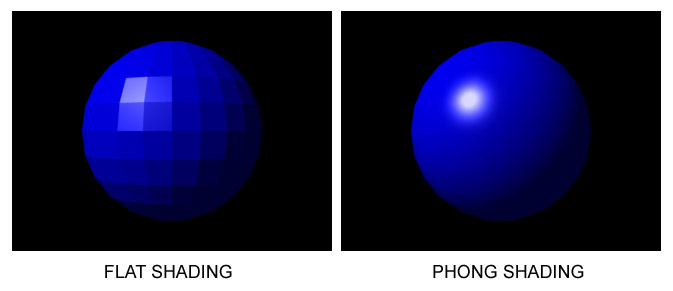
\includegraphics[width=\textwidth]{time_vs_quality}
    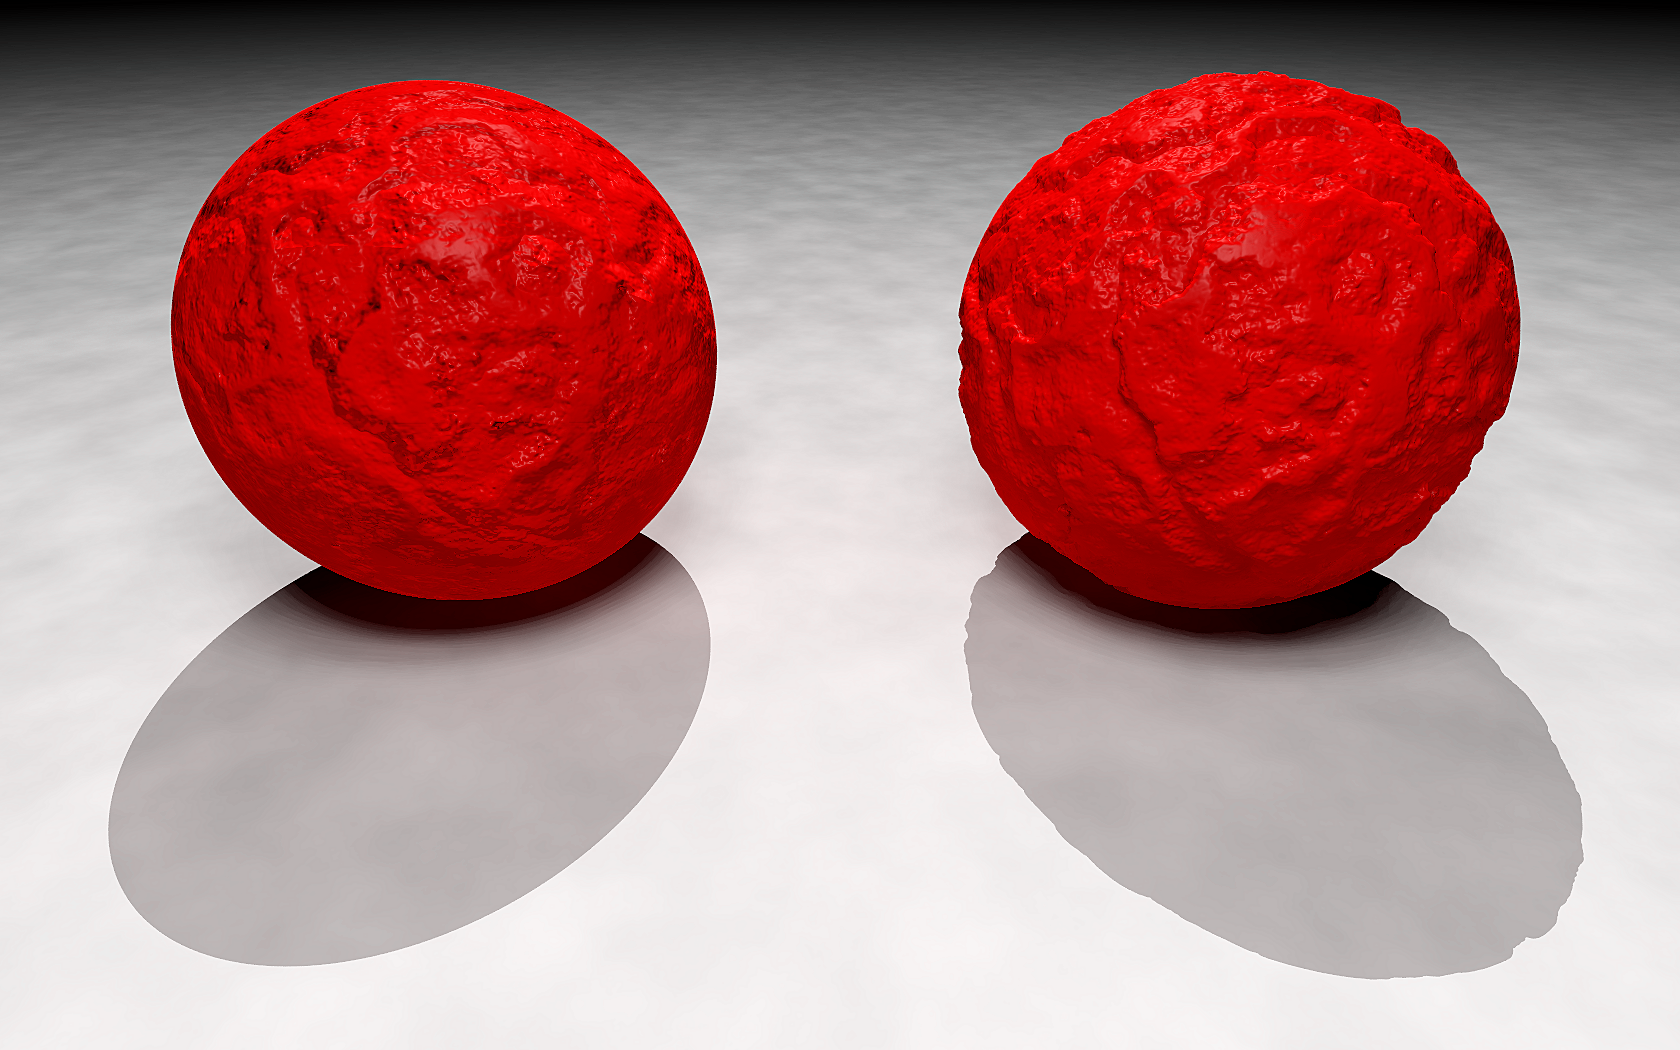
\includegraphics[width=\textwidth]{bumpmaps}
    \caption{Interpolation af flade-normaler kan få kantede figure til at få mere naturligt udseende.}
    \label{fig:tid_versus_kvalitet}
    % Demo der viser det samme http://math.hws.edu/graphicsbook/demos/c4/smooth-vs-flat.html
\end{figure}
\subparagraph{Rasterisering}
Den mest almindelige metode til at rendere miljøer med høj aktiv bruger interaktion er rasterisering. Rasterisering er også betegnelsen for at omdanne vector objekter til punkmatricer eller pixel-billeder (Se figur \ref{fig:pixelering}) Metoden virker ved at andvende linear transformationer på vektor objekter for at finde deres position på skærmen og derefter udfylde 2D polygonerne med farve, evt. baseret på forskællige lyskilder. Der kan dog simplificeres ved kun at andvende en ambient lys konstant. Rasterisering er også effektiv fordi grafikprocessore i computere er udviklet specifikt til at udføre matrix transformationer på store punktmængder.
\begin{figure}[H]
    \centering
    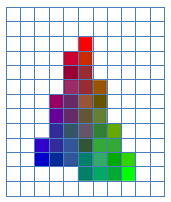
\includegraphics{rastarization_aprox}
    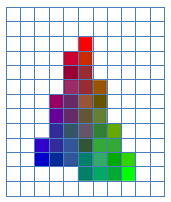
\includegraphics{rastarization_aprox}
    \caption{Pixelering der fremkommer når vektor objekter rastariseres.}
    \label{fig:pixelering}
\end{figure}
\subparagraph{Ray tracing}
% Kilder
% https://www.cs.unc.edu/~rademach/xroads-RT/RTarticle.html
% 
Raytracing er en metode som med relative simple regler, forsøger at andvende en fysisk model af lys, hvor fotoner spredes fra en lyskilde og rammer forskællige objekter indtil nogle få rammer øjet eller kamerarets optik. Raytracing simplificere ved at reducere problemet til kun at simulere de stråler der rammer vores øje. Dette gøres ved såkaldt \texit{backward ray tracing} hvorved man følger en stråle fra øjet, igennem computerskærmen og ind i vektormodellen hvor man tjekker for kollisioner mellem strålen og objekter. Ved kollision med reflektiktive objekter som metaliske overflader og gennemsigtige objekter som glas, vil strålen nu dele sig og følge f.eks gennem glasset men også følge en reflektiv vinkel for at udregne farven som den gennemsigtige/reflektive overflade har. For hver kollision følger man også en stråle mod alle lyskilder for at teste om der er objekter i vejen, således at kollisionspunktet ligger i skygge, da dette tages i betragtning som farven udregnes. Ved kollision med et mat objekt eller efter en forudbestemt antal reflektioner/refraktioner stopper udregningen og propagere tilbage igen.
\subparagraph{Radiosity}
% Kilder
% http://web.cs.wpi.edu/~matt/courses/cs563/talks/radiosity.html 
% http://www.cs.bath.ac.uk/~pjw/NOTES/75-ACG/ch5-radiosity.pdf
Hvor Rasterisering og raytracing udregner en pixels farve baseret på hvad man kan se igennem en skærmflade, så er radiosity en metode som er uafhængig af hvor kameraret er placeret og er af samme grund en af de mest tidskrævende metoder. (Måske er det muligt at precomputere modellen og så sende den til brugeren som kan interaktere med modellen via kameraret). Radiosity er baseret på en fysisk forståelse af lys interaktion med flader og fungere ved at alle flader absorbere en del af lyset der rammer dem og reflektere(radiates) resten som så går videre til at gentage processen for andre flader i scenen. Ved radiosity er lyskilder selv geometriske flader, hvilket gør det nemt at beskrive elementer som lamper og el-pærer. Karakteristisk for denne metode er såkaldt \textit{color bleeding}, hvor farver fra forskællige objekter smitter af på hindanden.
\begin{figure}[H]
    \centering
    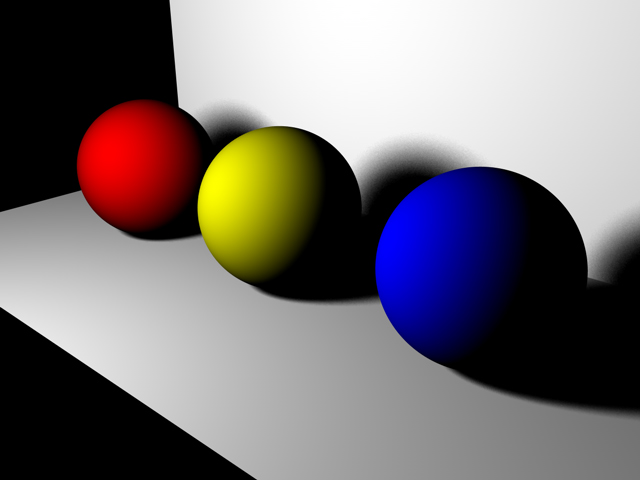
\includegraphics[width=6cm]{without_radiosity}
    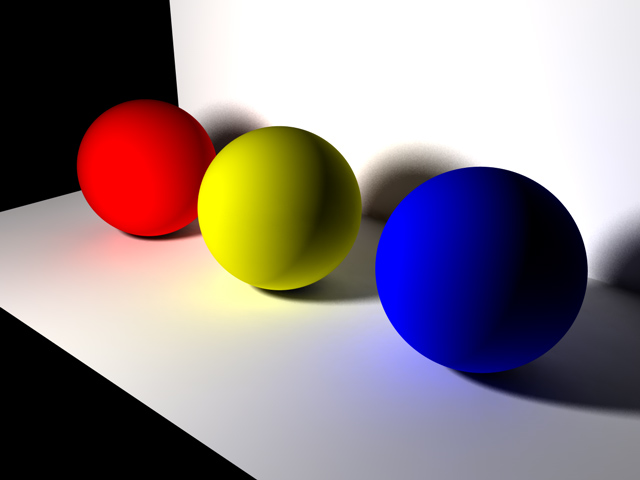
\includegraphics[width=6cm]{with_radiosity}
    \caption{\texit{Color bleeding} kan ses i billedet til højre.}
    \label{fig:colorbleeding}
\end{figure}

\clearpage


\section{Problemformulering}

Ud fra problemanalysen er vi blevet opmærksomme på følgende problem indenfor problemfeltet:
Det er et problem at kunden i en købssituation på e-butikker ikke kan visualisere, hvordan lys udbreder sig fra en lampe. Dette kan føre til fejlkøb af lamper, som påvirker både forbrugeren og e-butikken. For brugeren kan dette betyde irritation og i værste tilfælde kan det have sundhedsmæssige konsekvenser. For lampebutikker kan fejlkøb medføre utilfredse kunder og dårlig omtale. 

Dette fører os til det overordnede spørgsmål som vi ønsker besvaret i dette projekt:

\textit{Hvordan kan vi lave et værktøj til e-butikker, som vha.\ raytracing, visualiserer belysningen fra indendørslamper for kunderne?}

Herunder er der en række underspørgsmål, som ønskes besvaret:

\begin{enumerate}

\item \textit{Hvordan kan lampen visualiseres fra flere vinkler?}
\item \textit{Hvordan udbredes lyset fra en given lampe?}

\end{enumerate}


\renewcommand\refname{Bibliografi}
\begin{thebibliography}{99}

\section{Referencer}

\begin{thebibliography}{99}


\bibitem{kvalitativ_metode}
  Forklaring af kvalitativ metode,
  Den Store Danske.
  Set 25-11-2015.
  \url{http://www.denstoredanske.dk/Samfund,_jura_og_politik/Sociologi/Sociologisk_metodologi/kvalitative_metoder}

\bibitem{nummermetoden}
  Beskrivelse af nummermetoden, set 17-12-2015,
  \url{http://iva.ku.dk/refererkorrekt/tekshenvisninger/#Nummermetoden}

\bibitem{human_factors}
  Human Factors in Lighting, third edition,
  Peter R. Boyce, 2014.
  Sider 532-536.
  ISBN: 9781439874882.

\bibitem{ergonomi_arbejdsplads}
  Konsekvenser ved dårlig belysning på arbejdsplads mm.,
  ebscohost.
  Set 2-12-2015
  \url{http://web.b.ebscohost.com/ehost/detail/detail?sid=2898a5ec-e3ec-4bf2-b3b7-f4eb754cd767%40sessionmgr115&vid=0&hid=101&bdata=JnNpdGU9ZWhvc3QtbGl2ZQ%3d%3d#anchor=toc&db=buh&AN=7531667}

\bibitem{OSHA}
  Occupational Safety \& Health Administration,
  Set 16-12-2015.
  \url{https://www.osha.gov/}
  
\bibitem{CVS}
  Computer vision syndrom,
  gmj.
  Set 2-12-2015.
  \url{http://gmj.sljol.info/article/10.4038/gmj.v11i1.1115/galley/1023/download/}
  
\bibitem{ddo_visualisering}
  Definition af visualisering,
  Den danske ordbog.
  Set 27-10-2015.
  \url{http://ordnet.dk/ddo/ordbog?query=visualisere}
  
\bibitem{def_lys}
  Definition af lys,
  Videnskab dk.
  set 27-10-2015.
  \url{http://videnskab.dk/sporg-videnskaben/hvad-er-lys}
  
\bibitem{britannica_lys}
  Definition af lys,
  Britannica.
  Set 27-10-2015.
  \url{http://global.britannica.com/science/light}

\bibitem{integral_led}
  Om integral-led,
  integral-led.com.
  Set 2-11-2015.
  \url{http://www.integral-led.com/about-integral-led}
  
\bibitem{varm_kold}
  Definition af varm og kold lys,
  integral-LED.
  Set 27-10-2015.
  \url{http://www.integral-led.com/education/warm-white-or-cool-white}

\bibitem{american_heritage}
  American Heritage,
  The free dictionary.
  set 27-10-2015
  \url{http://www.thefreedictionary.com/lamp}

\bibitem{fysisk_kontra_online}
  The State of Retail 2015,
  Timetrade
  Sarah Wallace.
  Rapport udgivet i 2015.
  Side 22, figur 14.
  Copyright © 2015 by TimeTrade Systems, Inc.
  Set 3-11-2015.
  \url{http://www.timetrade.com/system/files/surveys/State_of_Retail_Report_Final_June15.pdf}

\bibitem{fortrydelsesret}
  Fortrydelse og returret,
  forbrug.dk.
  Set 28-10-2015.
  \url{http://www.forbrug.dk/Raad-og-rettigheder/Forbrugerleksikon/Fortrydelsesret}

\bibitem{ikea_returret}
  Ikeas returret,
  Ikea.
  Set 27-10-2015.
  \url{http://www.ikea.com/ms/da_DK/kundeservice/kundeservice_sporgsmaal_svar_kontakt_os.html?ICID=DKFOO_KONTAKT_230315}
  
\bibitem{ddo_ehandel}
  Definition af e-handel,
  Den Danske Ordbog.
  Set 26-10-2015.
  \url{http://ordnet.dk/ddo/ordbog?query=ehandel}

\bibitem{ddo_ebutik}
  Definition af e-butik,
  Den Danske Ordbog.
  Set 26-10-2015. 
  \url{http://ordnet.dk/ddo/ordbog?query=ebutik}

\bibitem{retsinformationen}
  Lov om forbrugeraftaler,
  Retsinformationen.
  Set 26-10-2015.
  \url{https://www.retsinformation.dk/forms/r0710.aspx?id=160666}

\bibitem{computergrafik_introduktion}
  A Short Introduction to Computer Graphics,
  Frédo Durand - MIT Laboratory for Computer Science.
  CSAIL.
  Set 5-11-2015.
  \url{http://people.csail.mit.edu/fredo/Depiction/1_Introduction/reviewGraphics.pdf}
  
\bibitem{Cylindo}
  Visual content and software as a service,
  Cylindo.
  Set 9-11-2015.
  \url{http://www.cylindo.com/}
  
\bibitem{rastarization} 
  Real-Time Massive Model Rendering, first edition, Sung-Eui Yoon, 2008. Side 31. ISBN: 9781598297928.

\bibitem{raytracing_for_begyndere}
  Ray Tracing: Graphics for the Masses, 
  Paul Rademacher of Department for Computer Science at the University of North Carolina at Chapel Hill.
  Department of Computer Science, University of North Carolina at Chapel Hill.
  Set 5-11-2015.
  \url{https://www.cs.unc.edu/~rademach/xroads-RT/RTarticle.html}

\bibitem{perspective_projection}
  Essential mathematics for games and interactive applications : a programmer's guide, second edition, James Van Verth \& Lars M   Bishop, 2008. Sider 212-236. ISBN: 9780080878614.
  
\bibitem{phong_paper}
  Illumination for computer generated pictures, Volume 18 Issue 6, Bui Tuong Phong \& Robert Ashenhurst, 1975. Sider 311-317. ISSN: 0001-0782.

\bibitem{stanford_phong}
  Raytracing, 
  CS148 AS3, Stanford University. 
  Set 01-12-2015.
  \url{http://graphics.stanford.edu/courses/cs148-10-summer/as3/instructions/as3.pdf}

\bibitem{tanner_helland}
  How to Convert Temperature (K) to RGB: Algorithm and   Sample Code,
  Tanner Helland.
  Set 04-12-2015.
  \url{http://www.tannerhelland.com/4435/convert-temperature-rgb-algorithm-code/}
  
\bibitem{charity_values}
  Blackbody color datafile, 
  Mitchell Charity. S
  et 04-12-2015.
  \url{http://www.vendian.org/mncharity/dir3/blackbody/UnstableURLs/bbr_color.htmle/}
  
\bibitem{tanner_helland_chart}
  Raw temperature vs RGB chart,
  Tanner Helland. 
  Set 09-12-2015.
  \url{http://www.tannerhelland.com/4435/convert-temperature-rgb-algorithm-code/raw_temperature_vs_rgb_chart/}

\bibitem{farvetemp}
  Beskrivelse af farvetemperatur, 
  Den Store Danske. 
  Set 13-12-2015.
  \url{http://www.denstoredanske.dk/It,_teknik_og_naturvidenskab/Elektricitet/Belysning/farvetemperatur}
  
\bibitem{solidworks}
  Liste af solidworks produkter, 
  solidworks. 
  Set 13-12-2015.
  \url{http://www.solidworks.com/sw/3d-cad-design-software.htm}

\bibitem{augmented_reality}
  Beskrivelse af augmented reality,
  Augmented Reality.
  Soha Maad
  Chapter 1, section 4
  ISBN 978-953-7619-69-5

\bibitem{artemides}
  Artemides Augmented Reality App, 
  Artemide.
  Set 14-12-2015.
  \url{http://www.artemide.com/blog/portfolio/the-new-version-of-artemide-augmented-reality-is-now-available/}

\bibitem{raytracingvsrastarizatioin}
  Fordele ved raytracing frem for rasterisering, set 16-12-2015,
  \url{http://www.tomshardware.com/reviews/ray-tracing-rasterization,2351-3.html}

\bibitem{softshadow}
  Beskrivelse af bløde skygger i raytracing, set 16-12-2015,
  \url{https://graphics.ethz.ch/teaching/former/seminar/handouts/Lang_SoftShadowVolumes.pdf}

\bibitem{rotationsmatricer}
  Weisstein, Eric W. "Rotation Matrix." From MathWorld--A Wolfram Web Resource, set 17-12-2015,
  \url{http://mathworld.wolfram.com/RotationMatrix.html}

%\bibitem{forbrugerportalen}
%  Definition af forbruger,
%  Forbrugerportalen
%  set 27-10-2015
  
%  \url{http://www.forbrugerportalen.dk/sider/artikel.asp?ID=13}


% \bibitem{prototyper_pdf}
%  Anvendelse af prototyper,
%  Teknologisk.dk
% set 27-10-2015
  
% \url{www.teknologisk.dk/_root/media/52285_Prototyping.pdf}

% \bibitem{fysiske_butikker}
% Forbrugere vil betale mere for varer i butikker,
% caltech.edu
% set 27-10-2015
  
% \url{http://www.caltech.edu/news/consumers-will-pay-more-goods-they-can-touch-caltech-researchers-say-1650}


% \bibitem{SolidWorks} 
%  3D CAD Software brugt af designere i IKEA,
%  set 17-11-2015
%  \url{http://www.3ds.com/products-services/solidworks/},
  
\end{thebibliography}
\clearpage

\clearpage

\documentclass[oneside,a4paper,titlepage]{article}
\usepackage{blindtext}
\usepackage[utf8]{inputenc}
\usepackage{pdfpages}
\usepackage{graphicx}
\usepackage{geometry}
\usepackage{float}


\begin{document}

\section{Beskrivelse - Hvordan forløb processen i P1}
% I skal beskrive jeres P1 projektproces så detaljeret som muligt. I må gerne komme ind på alle de aspekter I finder relevante. I skal komme ind på følgende områder:

Lige efter gruppedannelsen skete der ikke så meget i projektet, da vi var meget i tvivl om vores projektforslag. Projektforslaget var nemlig ikke fremstillet på samme måde som de andre. Under et af lektionerne til PV skulle vi i gruppen udfylde en række spørgsmål til f.eks.\ hvordan gruppen vil håndtere konflikter og hvordan vores samarbejdsaftale så ud, disse spørgsmål kan ses i bilag \ref{sec:samarbejdsaftale}. Der var også en lektion i PV, der handlede om at få styr på projektet, denne omhandler planlægning, værktøjer og roller \ref{sec:styr_paa_projektet}.\newline
I gruppen benytter vi os meget af "Peer-learning". Grunden til dette er at gruppens medlemmer har forskellige kompetencer og dette kan vi udnytte vi at hjælpe hinanden. Vi har hjulpet hinanden ved at et gruppemedlem laver en kort fremlæggelse på tavlen, så det andre gruppemedlemmer om ikke andet kan få en nogenlunde forståelse og et godt udgangspunkt til viderearbejde.
Til konflikter som f.eks.\ overskredte deadlines eller at komme for sent til gruppearbejde har vi været meget large. Enten er deadlines blevet rykket eller man er blevet tvunget til at give kage. 

Til disse spørgsmål havde vi til samarbejdsaftalen aftalt at møde 8:15 og derefter arbejde fra 8:30 til 16:15. Efterhånden som projektet forløb blev lavet om til at møde 8:30 og derefter til vi ikke rigtigt gad mere og havde nået det vi ville på dagen. Vi har ikke udarbejdet en fast tidplan, men der er derimod en consensus om at der er frokost klokken 12. Der er dage hvor frokosten rykker sig, hvis vi glemmer tiden når vi har været meget fokuseret på arbejdet. Vores skriftlige samarbejdsaftale er derfor ikke særlig lang, vi har dog mange mundtlige aftaler og gensidig respekt for hinanden. 

Vi lavede en Bilbin rolletest, hvor vi på baggrund af denne bestemte gruppens kontaktperson og hvem der skulle træde til som leder hvis det blev nødvendigt. Vi har derfor ikke haft en fast projektleder, da vi mente du var nødvendigt og formentlig fordi på daværende tidspunkt vil de være lidt akavat at skulle agere chef over for de andre i gruppen.

Til samarbejde med vores vejledere, gav begge vejledere os en papir om hvilke krav de havde til samarbejdet. Disse papirer har fungeret som vores samarbejdsaftale med vejlederne. De omhandlede bl.a.\ i hvilken format arbejdsblade skulle sendes i, hvor lang tid de skulle have til at læse dem og at kun referentens pc skulle være åben. Inden et vejledermøde havde vi lavet en agenda som på forhånd blev sendt til vejlederen. Vi havde to former for vejledermøder, den ene var at vi sendte vores arbejdsblade hvorefter vi vil få feedback i form af kommentarer over mail. Den anden var det mere traditionelle vejledermøde hvor vejlederen havde udprintet rapport og kommentarerne blev diskuteret face-to-face. 

Da vi skulle til at lave den initierende problemstilling lavede vi en overordnet tidsplan til hvornår vi skulle have de store emner gjort færdig. Ud fra denne sørgede vi at give os selv opgaver og deadlines løbende så dette mål ville blive opfyldt. 

Når vi skulle uddele opgaver til os selv, havde vi skrevet opgaverne op og derefter kunne man selv sætte sig på noget eller blive sat på noget. Motivering i gruppen kom løbende, vi motiverede hinanden og hjalp til, så personen ikke kørte død i skrivearbejdet, jokes og sociale pauser hjalp meget med dette. Hver morgen lavede vi dagsordner til hvad vi lave den dag, på den måde, dette hjalp med at overholde tidsplanen. Til at organisere vores arbejde har gruppen benyttet sig af Trello, da det er meget nemt at lave nye kort med opgaver og man kan hurtigt få oversigt over dem. Som det kan ses på figur \ref{fig:trello} kan man se hvem der er på hvilke opgaver og hvor langt opgaven er fra at være færdig.

\begin{figure}[H]
    \centering
    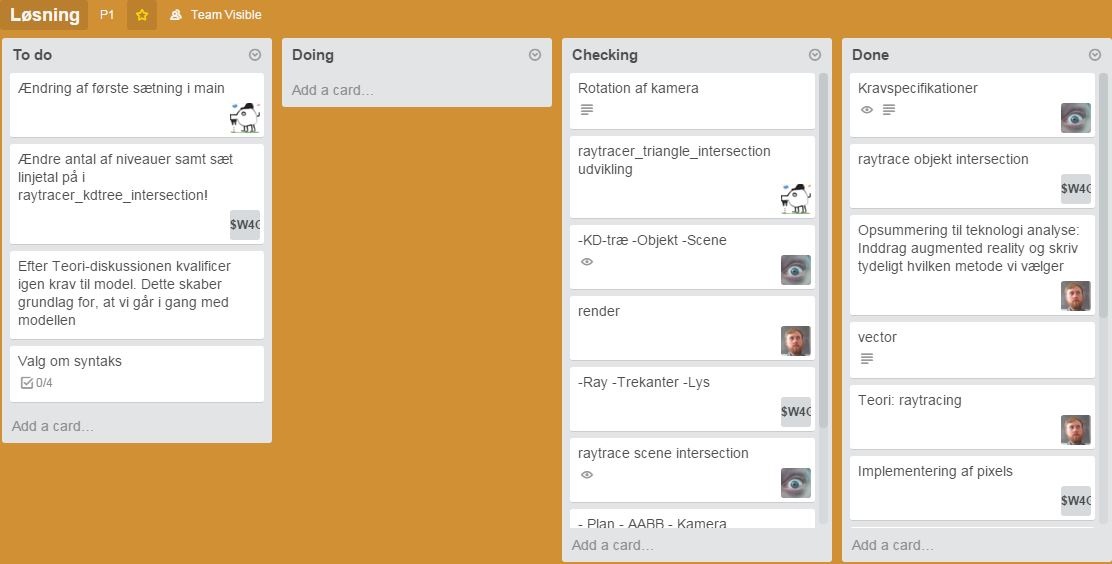
\includegraphics[width=10cm]{../graphics/trello}
    \caption{Et udklip fra vores løsningsboard på Trello}
    \label{fig:trello}
\end{figure} 

Vi brugte Git til vores versioncontrol således at alle hurtigt den hente den nyeste version, Git blev også brugt til at holde styr på koden. I forbindelse med projektet kontaktede vi flere personer og virksomheder, vi skrev til ti lampebutikker, to designere og IKEA. Ansvar for denne kommunikationen lagde på kontaktpersonen, som var ansigtet ud ad til. 

Opgaverne uddeles for de meste med først til mølle, men der bliver stadigt taget højde for omfanget af opgaven så det ikke ender med at en person har en 30 minutters opgave mens en anden har en to timers opgave. Enten vil personen med den lille opgave få noget mere at lave eller den store opgave opdeles og laves med en mere person. Vi holder korte og uformelle møder her og der, hvor vi kommer med en status på mangler og lignende i rapport eller koden. Da møderne i sig selv er så uformelle, er der ingen mødeleder eller runde om border, hvis man har noget at byde ind med byder man ind. 
Vi har ikke haft en seriøs snak om hvad vi forventer af hinanden, det ligger meget implicit når vi arbejder. Der er dog nogle forventninger, der er blevet sagt f.eks.\ at vi møder til tiden og at man laver det man er blevet bedt om. Ambitionen ligger selvfølgelig højt, vi vil gerne lave noget vi kan stå inde for og gøre vores bedste. Vi forventer ikke at gruppemedlemmer tager med på bar eller andet, hvis de ikke har lyst. Det er noget man selv bestemmer om man vil eller ej, vi vil dog stadig spørge efter det og prøve at få en person til komme med, da vi kun har kendt hinanden i under et halvt år. 

Vi hjælper hinanden med gruppeopgaver til det forskellige kurser, i programmering foregik dette ved at vi fælles skrev koden og viste den på en projekter. I matematik lavede vi opgaver selv så meget som muligt, men man kunne frit slå sig sammen med en anden eller spørge, vi sørgede for at alle havde en forståelse for hvordan opgaven skulle løses. Hvis en forstod noget som nogle andre ikke gjorde holdte denne person ofte en kort fremlæggelse på tavlen så de andre havde en godt nok forståelse til at de kunne lave opgaverne. 

En af de arbejdsprocessor som vi havde i gruppen var, at vi hver morgen lavede en dagsorden for dagen. Vi vil i dette afsnit kort forklare og illustrere nogle af de dagsplaner som
vi havde under P1. 

Her er et par eksempler på dagsordner i løbet af projektet:
\paragraph{Dagsorden 9/10/15:}
\begin{itemize}
  \item Brainstorm
  \item Diskution af spørgsmål til styringsgruppe mødet.
  \item Agenda
  \item Find de programmer vi vil bruge til projektarbejde, heraf undersøg Trello, og github.
  \item Opsummering og afrunding  af dagen.
\end{itemize}
Her ses en typisk dagsorden for starten af projektet, hvor vi brugte lang tid på at diskutere hvilket emne vi ville arbejde med, samt at få styr på praktiske ting som programmer til fildeling.

Et andet eksempel på en dagsorden kunne se således ud:
\paragraph{Dagsorden 20/11/15:}
\begin{itemize}
  \item Agenda til Annette
  \item Planlæg
\end{itemize}
I slutningen af projektet var der fokus på at samle trådene og en dagsorden så derfor ofte således ud:

\paragraph{Dagsorden 14/12/15:}
\begin{itemize}
  \item Revidere afgrænsning af løsningsforslag.
  \item Skrive afsnit om rotationsmatricer i udviklingsafsnittet.
  \item Fordele og ulemper ved augmented reality.
  \item Skitse til Phong.
  \item Ret sekvensdiagram.
  \item skriv testafsnit færdigt.
\end{itemize}
Her ses der en dagsorden lavet nogle dage før projektafleveringen, og her er der fokus på at rette eventuelle mangler.
%læreprocessen (herunder problemorienteringens røde tråd)



%Det er vigtigt at I venter med at analysere jeres erfaringer til efter at I er færdige med at beskrive dem ! 


\section{Vurdering - Hvordan gik det}
\begin{itemize}
  \item Opgaveuddeling ved hjælp af Trello gik godt i starten og knap så godt i slutningen af projektet.
  \item Git som versioncontrol var rigtigt god til at holde styr på koden, men knap så god til latex.
  \item Dagsordnerne gik godt, men nogle gange var de meget korte og upræcise.
  \item Grupperolletesten er slet ikke blevet brugt udover at give os selv kendskab til hvilke roller vi har.
  \item Gruppesamarbejdet gik okay, der var nogle gode ting og nogle dårlige ting. 
  \item Vejledersamarbejdet gik godt.
  \item Samarbejdet med erhvervslivet hjalp meget med god viden til viden rapporten, selvom vi blev afvist af IKEA.
  \item kommunikationen i gruppen er hovedsageligt god og samtaler kan godt afsluttes når vi skal arbejde. 
  \item Nogle i gruppen kan være ufokuseret og følger ikke med om morgenen når dagsordenen laves, hvilket ofte ender i at den person ikke laver noget.
  \item Gruppens konflikthåndtering har været meget dårlig.
  \item Vi har været dårlige til at stå op og "skælde" en person ud hvis de ikke følger med.
  \item Gennemgang af rettelser på projekter var godt.
  \item Fællesregning af gruppeopgaver fra kurser var godt.
\end{itemize}

% Trello er godt med mindre boards, godt til hjemmeopgaver
% Git er godt til koden, men måske ikke fan til latex, to forskellige repository
% Mere konkrete dagsordner, som bliver tjekket op på. evt. navne på opgaven
% Har ikke brugt grupperolletesten, andet end få et kendskab til hvilke roller der er, og hvilke vi er. 
% Gruppesamarbejde gik okay
% Vejledersamarbejde gik godt
% Samarbejde med erhvervsliv gik godt 

Hvordan er kommunikationen i jeres gruppe ? Er der nogle der taler hele tiden ? Er der nogen der aldrig siger noget ? Bruger gruppen uforholdsvis lang tid på diskussionerne ? Hvorfor ?

%Når I er færdige med at beskrive hvad I gjorde, skal I vurdere hvordan det gik. Med andre ord: Hvad gik godt i P1? Hvad gik dårligt i P1? 

\section{Analyse – Hvorfor gik det som det gik?}
%Dernæst skal I analysere jeres arbejdsprocesser og få klarlagt hvorfor noget gik godt mens andet gik dårligt. Med andre ord: Hvad er det for faktorer, som har indvirket på arbejdsprocesserne? 

\section{Syntese – Gode råd til P2}
% samarbejdsaftale, snakke sammen om konflikter og engagement

%Hvis jeres vurdering og analyse skal bidrage til at forbedre jeres evne til at håndtere det
%problemorienterede og projektorganiserede gruppearbejde, skal I til slut konkretisere jeres erfaringer i nogle ’Gode råd’ til jer selv og jeres medstuderende. En god måde at formulere sådanne gode råd på er som en *start-stop-fortsæt*-liste, dvs. en liste med følgende tre sektioner:
%– Dette vil vi begynde at gøre i P2, som vi ikke gjorde i P1 
%– Dette vil vi ikke gøre i P2, som vi gjorde i P1
%– Dette vil vi fortsætte med at gøre (gerne anderledes og bedre) i P2, som vi også gjorde i P1
%Det er en god idé at tage ét område ad gangen og gøre det færdigt. De ’Gode råd’ skal være konkrete og operationelle, så de fører til reelle forbedringer i P2. 


Spørgsmål til inspiration
Når I skal skrive P1-procesanalysen kan I lade jer inspirere af spørgsmålene herunder, men I må
gerne medtage andre emner, som I mener har haft betydning for jeres arbejdsprocesser.
Projektplanlægning
Har alle i gruppen samme opfattelse af hvad projektplanlægning er ? Find ud af det.

Hvad vil I foreslå til planlægning og styring af et P2 projekt ?

Samarbejdet i gruppen

Hvilke forventninger har I til samarbejdet i P2 ? Hvordan skal de blive opfyldt ?

Samarbejdet med vejlederne
Hvilken type respons ønsker I fra vejlederen ?
Hvilken type vejledning har I modtaget ? Var det hvad I ønskede jer ?
Hvilke forventninger vil I stille til jeres vejledere i P2 ?

Læreprocesserne
Hvordan hjælper I hinanden med at løse opgaver i kurserne ?
Hvad gør I hvis I ikke forstår det der bliver sagt/eller står i bogen ?
Hvordan lærer du bedst ?
Hvordan har I brugt resultaterne af jeres individuelle læringstest ?
Hvordan hjælper/stimulerer vejlederen jeres læreprocesser ?
Hvilken læringsstrategi er bedst til kurser ?
Hvilken læringsstrategi er bedst til projektarbejde ?


\clearpage
\section{Bilag}

\subsection{Belbins teamroller}
\label{sec:styr_paa_projektet}
\section*{PV – Få styr på projektet}
\subsection*{Planlægning}
\begin{itemize}
  \item Initierende problem – 15 / 10
  \item Problemanalyse \& problemformulering – 14 / 11
  \item Løsning (metode) – 14 / 11
  \item Udvikling – 7 / 12
  \item Dokumentation – 12 / 12
  \item Konklusion – 14 / 12
  \item Afslutning og aflevering – 18 / 12
  \item Procesanalyse – 22 / 12
\end{itemize}

\subsection*{Værktøjer}
\begin{itemize}
  \item Trello
  \item Github
  \item Latex
  \item Google docs
\end{itemize}
Trello er til opgaveadministration.
Git er til version-control.
Docs er til fællesrettelser.
Latex er det system vi skriver rapporten i.
\subsection*{Roller}
\begin{itemize}
  \item Kontaktperson: Lasse
  \item Referent: Skiftende rolle
  \item Ordstyrer: Skiftende rolle
  \item Leder: Anton og Morten
\end{itemize}
Gruppen har taget en rollemodels test: \newline
Kristian Træhold: Formidler og Specialist. \newline
Christian Grunberg: Formidler og Organisator.\newline
Mathias Ibsen: Formidler og Specialist.\newline
Lasse Gadegaard: Organisator, kontaktskaber og formidler.\newline
Mathias Pihl: Organisator og specialist.\newline
Morten Rask: Organisator, koordinator, opstarter, afslutter, specialist.\newline
Anton Christensen: Koordinator, opstarter.\newline

\subsection*{Rollebeskrivelser}
Formidler: Social personlighed som er meget diplomatisk og løser konflikter.
Specialist: Har en stor faglig viden indenfor et område. Fokuserer på sit arbejde.
Organisator: Sørger for at tingene er i orden, og at vi har en tidsplan.
Kontaktskaber: Social person der holder styr på kommunikation, og alt det formelle.
Koordinator: Leder som tager beslutninger, og uddelegerer opgaver
Opstarter: Er god til at sætte folk i gang, og vil hele tiden lave noget
Afslutter: En der kan samle trådene, og ikke lader et projekt løbe ud af tangenter
Idémand: En person som altid ser nye muligheder og er en god debatstarter.

\begin{figure}[H]
   \centering
   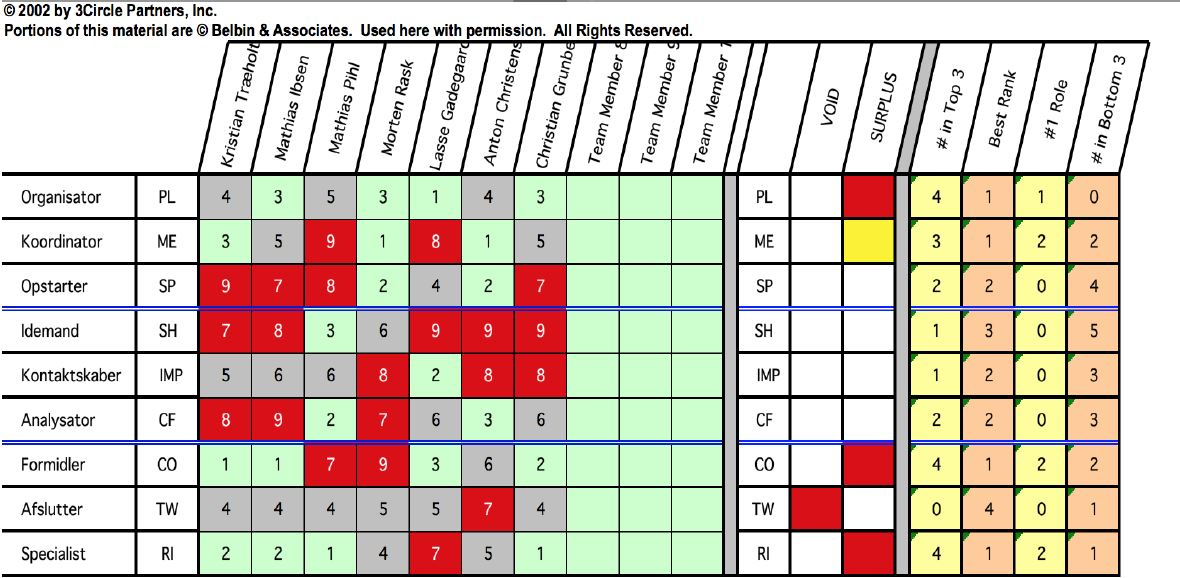
\includegraphics[width=10cm]{../graphics/rolletest}
   \caption{Resultatet af rolletesten}.
\end{figure}

\subsection*{Kommentar til skema:}
Vi kan se, at der generelt er en fin fordeling af roller, hvor den eneste som ikke er grøn er ”afslutter”, men her ses der at mange gruppemedlemmer har denne som 4 og 5 priotet. Det er derfor oplagt at tage denne i fællesskab. Derudover har vi 3 roller der er i SURPLUS. Her skal vi være opmærksom på, at der ikke bliver lavet for meget dobbeltarbejde, og at vi alle går i samme retning.

\subsection{Samarbejdsaftale mm.}
\label{sec:samarbejdsaftale}

\section*{Hvordan benytter gruppen resultaterne fra læringsstiltestene til at gruppemedlemmerne lærer bedre ”til og fra hinanden” (Peer læring)?}
Vi har fået en forståelse for at folk lærer og opfatter tingene på forskellige måder. Vi skal derfor være åbne for forskellige forslag, og have en accept for at folk lærer på forskelligt. Derudover skal vi inkorporere de forskellige læringsmetoder i vores gruppearbejde, hvor personer der f.eks. lærer bedst ved ”forklaring” – også får en mulighed for at forklare hvad personen har lært for andre.
\section*{Hvad vil i gøre i gruppen, hvis der opstår konflikter, som kræver en løsning?}
Vi skal finde frem til kernen af konflikten. Vi diskutere efterfølgende problemet, hvor vi har en ordstyrer som styrer slagets gang, og alle får derefter lov til at udtrykke deres mening/holdning om problemet. Derefter kan man finde eventuelle ligheder og forskelle, og derudfra finde en løsning på konflikten.
\section*{Hvordan ser gruppens samarbejdskontrakt ud?}
Vi møder hverdag kl 8:15 og begynder gruppearbejdet 8:30. Hvilket vil sige, at man har 15min til ”fri leg” – og sociale samtaler.
Normal arbejdsdag: 8:30 – 16:15 med mulighed for ændringer hvis ALLE er enige.
Vi vil lave et mål for hver dag. Altså en dagsorden for hvad der skal nås.
Man SKAL informere ”inden” mødetid hvis man ikke kan møde til tiden.
\section*{Vejleder:}
At vi foreslår, at vores arbejdspapirer bliver delt over google docs. og vejlederen har derefter mulighed for at kommentere i google docs. Vi laver en redigeringsaftale med vejlederen.
Lav en Agenda til hver møde
\clearpage
\subsection{Mail korrespondence}
Fra: XX \newline
Sendt: 6. november 2015 13:36 \newline
Til: Lasse Fribo Gadegaard\newline
Emne: SV: Semesterprojekt om lamper - AAU\newline
Hej
 
Det at se en lampe i 3D gør ikke at man ser lyset. Nogle af vores producenter laver allerede 3D modeller af deres lamper og endda sådan at man kan se lampen med lys i. Jeg har lige vedhæftet Artemides udgave af fremgangsmåden.

Men derfra til at se hvordan lyset er i et konkret rum hvor farver, højde mv. har indflydelse på lyset gør at det bliver en ekstrem kompleks størrelse der kræver komplicerede belysningsberegningsprogrammer som f.eks. DIALux. Lysberegning handler primært om lysmængde og ikke om lyseffekt.

Kunder har svært ved at forstå er hvilken lyseffekt lampen giver. Det er jo to-siddet. Dels vil de se hvordan lampen ser ud i rummet og dels vil de se hvordan lyseffekten er. Første del klarer flere producenter. Hvis man så bagefter at man har sat lampen ind som 3D model burde man lave et lag over billedet hvor producenten så har taget et billede af et rum hvor man kan se skygger mv. Eks Tom Dixon. Det er det jo ikke lampe man køber men ofte lyseffekt og lampe handler jo om at forme lyset og lave skygger. At sætte en Tom Dixon lampe ind i et rum gør ikke at du kan se skyggerne.

Det er blevet en kompliceret proces at producere en lampe ift. EU lovgivning i dag så jeg har svært ved at se at producenterne vil koste endnu flere penge til produkter til privatmarkedet som måske kun køber en lampe til 3000 kr. som ofte kun interesserer sig for den laveste pris og ikke den bedste service og rådgivning. Så producenters incitament til ligge investeringer hos privatkunder er meget begrænset. Mange laver end ikke et fritskravet billede af deres lampe. Og igen Tom Dixon anvender en klar halogenlyskilde. Hvis du sætter en klar kultrådslyskilde hvor filamentet er længere giver forsat skygger men på en blødere måde da lyset er delt ud på en større overflade. Hvis du sætter en mat lyskilde i forsvinder skyggerne næsten helt. Pludselig er løsningen bare komplekst og når en producent så har 4000 varenumre. Samme lyskilder laves så i 3 farvetemperaturer. Med vores adgang til varesortiment giver det 2 mio. billeder dokumenter som skal indhentes. Så er vi der hvor det begynder ikke at hænge sammen tidsmæssigt når nethandlen handler om at være først ift. googlesøgninger mv. Hvem har lyst til at give bedste rådgivning ift. lyseffekter hvis man ender på side 20 når folk søger på google?  

Løsningsforslag modtages derfor med kyshånd da kompleksitet er desværre nem at se. 

I må selvfølgelig også gerne vores udtagelser.  

Med venlig hilsen / best regards

XX\newline
Belysninskonsulent

\noindent\makebox[\linewidth]{\rule{\paperwidth}{0.4pt}}

Fra: Lasse Fribo Gadegaard [mailto:lgadeg15@student.aau.dk] \newline
Sendt: 6. november 2015 11:19\newline
Til: XX\newline
Emne: SV: Semesterprojekt om lamper - AAU

Hej 
 
Vi er meget glade for at I vil bidrage til projektet. Indtil videre har vi analyseret problemet: 
Forbrugeren kan ikke visualisere, hvordan lyset udbreder sig fra en lampe uden at købe og installere lampen. 

I problemanalysen har vi undersøgt interessenter, begreber, placering og teknologier til problemet. 

Ud fra dette har vi valgt at fokusere på e-butikker, der sælger indendørs lamper til brug i erhverv eller private hjem. 

Vi har netop udarbejdet den endelige problemformulering, hvor udkastet lyder som følgende:
Hvordan kan man lave et værktøj til e-butikker som vha. raytracing*, visualiserer belysningen fra indendørs lamper for kunderne? 

* En teknik til at simulere lys og lave et billede af en 3D-model. 

Vi skal nu til at udvikle en løsning til problemet, og hertil har vi lavet en simpel skitse (Se vedlagt billede) af den ide vi har på nuværende tidspunkt. 
 
Som vist på skitsen, er ideen at lave et produkt som gør det muligt for kunderne at se nogle lamper og deres belysning i et interaktivt 3D-billede på e-butikken. 

Vi tænker at forbrugeren skal kunne gøre følgende: \newline
 - Vende og dreje billede, så de kan se lampen og belysningen fra flere vinkler. \newline
 - Se lampen med forskellige pærer (evt. angive farvetemperatur i Kelvin) \newline
 - Skifte den kontekst som lampen visualiseres i (f.eks. forskellige rum/møbler)

Pga. tidsbegrænsning forventer vi ikke at lave hele løsning, som produkt, men blot implementere de mest studierelevante dele. 

Dog skal vi stadigvæk præsenterer en færdig løsning i rapporten. 

Det vi nu ønsker jeres respons på, er følgende
 - Jeres tanker omkring ideen, som løsning på problemet.\newline
 - Forslag og ønsker til forbedringer af ideen. \newline
 - Jeres accept til, at vi i rapporten må inddrage jeres udtagelser anonymt.

Med venlig hilsen,\newline
Lasse Gadegaard
 
På vegne af \newline
Gruppe B2-28\newline
Software, AAU
 
\noindent\makebox[\linewidth]{\rule{\paperwidth}{0.4pt}}

Fra: XX \newline
Sendt: 5. november 2015 15:43\newline
Til: Lasse Fribo Gadegaard\newline
Emne: SV: Semesterprojekt om lamper - AAU\newline
Hej Lasse

Det lyder til at være et meget spændende projekt.
 
Som primær detailforretning med projektafdeling lever vi af konsulentarbejde ved at give rådgivning omkring hvordan lys forandre sig ift. til lofthøjde, farver, armatur, lyskilde foruden at der er en subjektiv mening om hvad godt lys er.

Der er overraskende mange der gerne vil se lyset inden de køber lamper. Man kan dog undre sig ovre at samme kunde køber både køleskabe, vaskemaskiner mv. uden at stille krav til at prøve tingene før de køber varerne selv om disse produkter koster lige så meget som de lamper vi sælger. Kunder har åbenbart et specielt forhold til lys. 

Har i allerede valgt teori, metode og empiri? 

Jeg tror godt vi kan hjælpe jer. Eneste krav er at data herfra bliver anonymiseret og vi får et eksemplar af opgaven når den er skrevet.

God dag

Med venlig hilsen / best regards\newline
XX\newline
Belysningskonsulent

\noindent\makebox[\linewidth]{\rule{\paperwidth}{0.4pt}}

Fra: Lasse Fribo Gadegaard [mailto:lgadeg15@student.aau.dk] \newline
Sendt: 5. november 2015 15:06\newline
Til: XX\newline
Emne: Semesterprojekt om lamper - AAU
 
Hej XX
 
Vi er en gruppe på Aalborg Universitet, som er i gang med et projekt om visualisering af lamper.
 
Vi arbejder med følgende problemstilling:
"Forbrugeren kan ikke visualisere, hvordan lyset udbreder sig fra en lampe uden at købe og installere lampen." 

Vi har fokus på e-handel, og ønsker at tilbyde e-butikken et værktøj som gør det nemmere for kunderne at visualisere, hvordan lyset breder sig ud fra en lampe (f.eks. hvilke skygger, mønstre og farver som lampen udsender). 

Derfor søger vi nu e-butikker, som ønsker at bidrage med viden og informationer omkring e-handel med lamper.  

Hvis I er interesserede i at medvirke i projektet, så skriv venligst tilbage på mail: lgadeg15@student.aau.dk 

Med venlig hilsen,\newline
Lasse Gadegaard\newline
På vegne af\newline
Gruppe B2-28\newline
AAU, Software

\subsection{Brainstorm}
\begin{figure}[H]
   \centering
   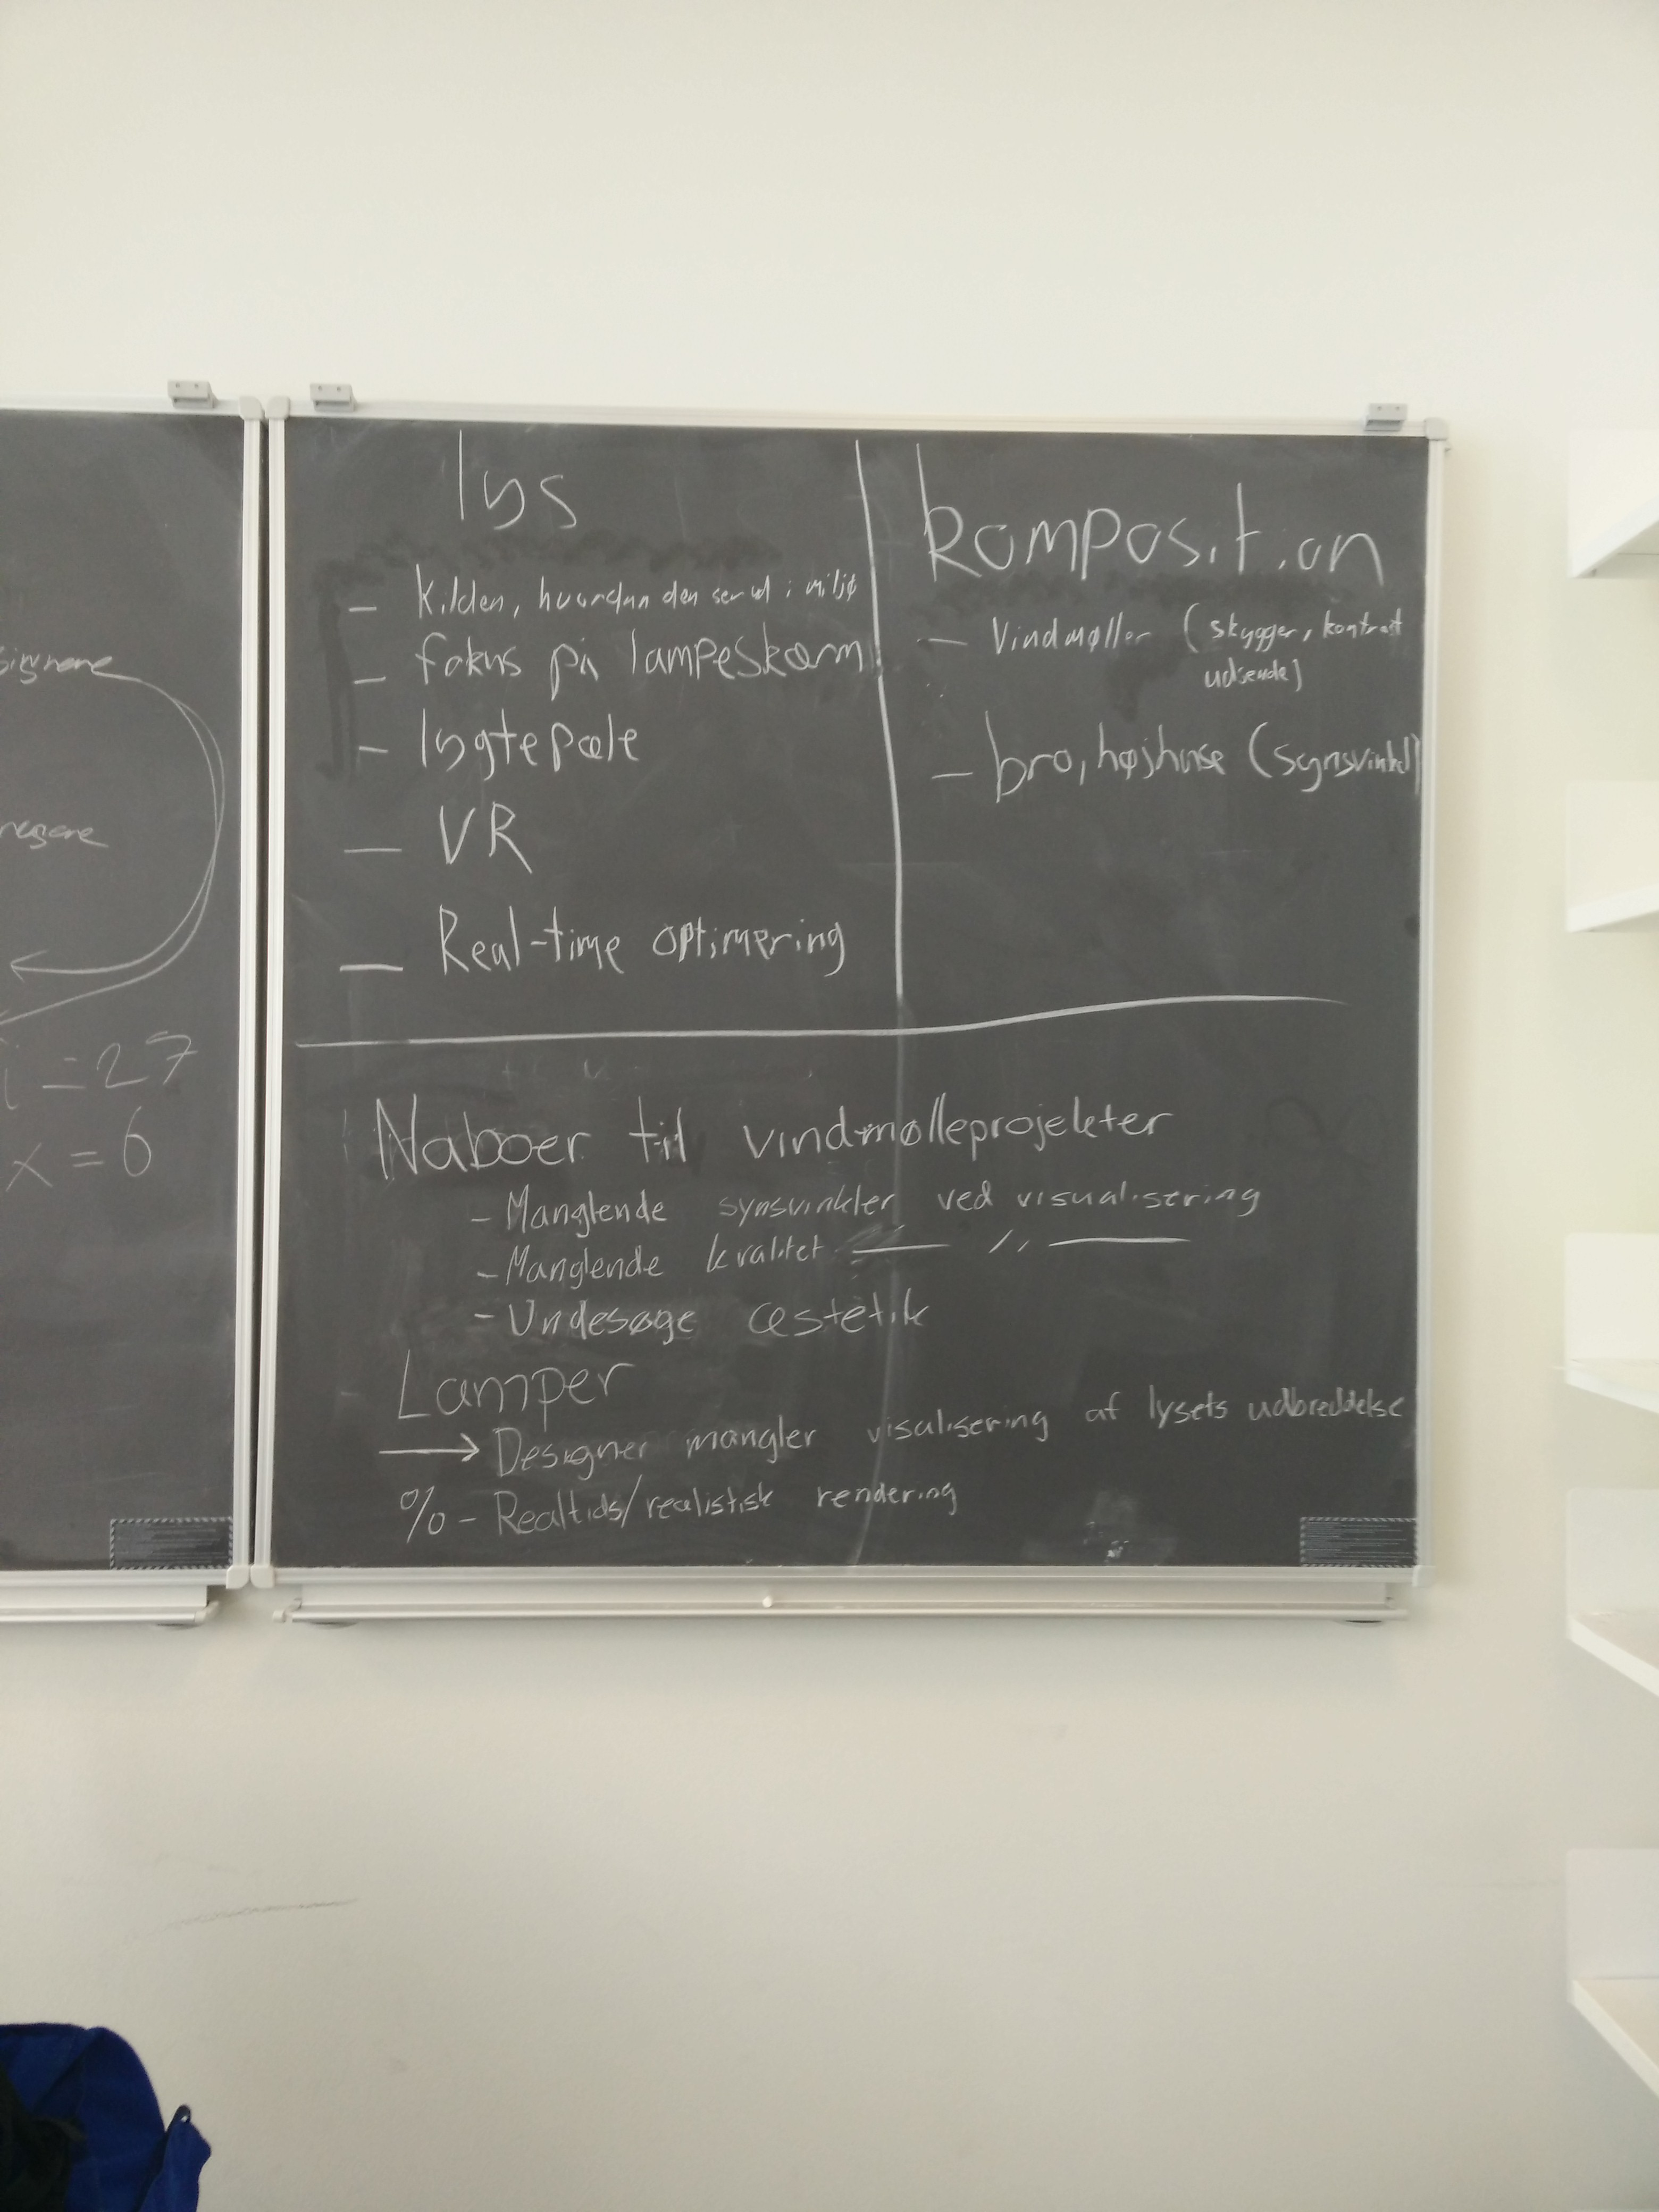
\includegraphics[width=10cm]{../graphics/brainstorm_1}
   \caption{Billede af første brainstorm}.
\end{figure}

\subsection{Dagsorden}
\begin{figure}[H]
   \centering
   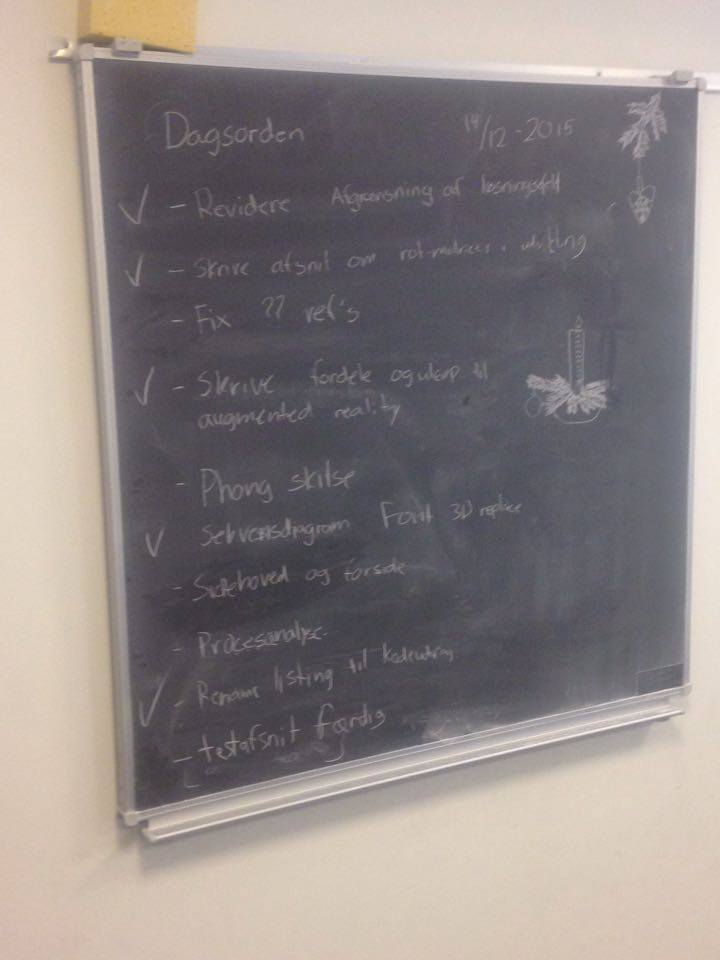
\includegraphics[width=10cm]{../graphics/dagsorden}
   \caption{Billede af en god dagsorden}.
   \label{fig:dagsorden}
\end{figure}

\end{document}


\end{thebibliography}
\end{document}
